\documentclass{standalone}
%
\usepackage{tikz}
\usetikzlibrary{backgrounds}
\usetikzlibrary{calc}
\usetikzlibrary{decorations.pathmorphing}
\usepackage{xcolor}
\usepackage{ifthen}
%
\definecolor{space}{HTML}{0A2543}
\definecolor{earth}{HTML}{0089FA}
\definecolor{dida}{HTML}{FFDE00}
\definecolor{title}{HTML}{FBA706}
%
\usepackage{fontspec}
\setmainfont{Open Dyslexic}
%
\title{Il messaggio di Arecibo}
\begin{document}
	\tikzset{
		partial ellipse/.style args = {#1:#2:#3}{insert path={+ (#1:#3) arc (#1:#2:#3)}},
		arecibo/.pic = {
			\foreach \i in {0,1,3,4}
			\draw[color=space, fill=red, ultra thick] (2+\i,0) rectangle (3+\i,1);
			\foreach \i in {0,1,2}
			\foreach \j in {0,1,2,3,4,5,6}
			{\ifthenelse{\j<3 \AND \i=1}{}{\draw[color=space, fill=red, ultra thick] (3+\i,1+\j) rectangle (4+\i,2+\j);}}
			\draw[color=space, fill=red, ultra thick] (4,8) rectangle (5,9);
			\draw[color=space, fill=red, ultra thick] (4,9) -- (4,10) -- (5,10) -- (5,9.4) -- (4.8,9.4) -- (5,9.3) -- (5,9) -- (4,9);
			\foreach \i in {0,1,2}
			\draw[color=space, fill=red, ultra thick] (\i,5+\i) rectangle (1+\i,6+\i);
			\foreach \i in {0,1,2}
			\draw[color=space, fill=red, ultra thick] (9-\i,5+\i) rectangle (8-\i,6+\i);
		},
		cross/.pic = {
			\foreach \i in {0,1,2}
			{\draw[color=space, fill=earth, ultra thick] (0.5+\i,0-\i) rectangle (1.5+\i,-1-\i);
				\draw[color=space, fill=earth, ultra thick] (3.5-\i,0-\i) rectangle (2.5-\i,-1-\i);}
		},
		ax/.pic = {
			\foreach \i in {0,3}
			\foreach \j in {0,1}
			\draw[color=space, fill=earth, ultra thick] (0+\i,-3-\j) rectangle (1+\i,-4-\j);
		},
		dna/.pic = {
			\pic at (0,0) {cross};
			\pic at (0,0) {ax};
			\pic at (0,-5) {cross};
			\pic at (0,-7) {cross};
			\pic at (0,-7) {ax};
			\pic at (0,-12) {cross};
		},
		cluster/.pic = {
				\foreach \i in {1,2,...,200}{
					\newcommand{\cX}{0}
					\newcommand{\cY}{0}
					\newcommand{\cR}{4.5}
					\pgfmathparse{70*rnd+30}
					\edef\tmp{\pgfmathresult}
					\pgfmathrandominteger{\x}{-450}{450}
					\pgfmathrandominteger{\y}{-450}{450}
					\pgfmathparse{0.01*\x}\let\x\pgfmathresult
					\pgfmathparse{0.01*\y}\let\y\pgfmathresult
					\pgfmathparse{ifthenelse((\x-\cX)^2 + (\y-\cY)^2 <= \cR^2,"red!\tmp!yellow","space")}
					\fill[\pgfmathresult] (\x,\y) circle (0.1);
				}
		},
		monster01/.pic = {
			\fill[green] (0,0) -- (0,1.5) -- (0.5,1.5) -- (0.5,2) -- (1,2) -- (1,2.5) -- (1.5,2.5) -- (1.5,3) -- (1,3) -- (1,3.5) -- (1.5,3.5) -- (1.5,3) -- (2,3) -- (2,2.5) -- (3.5,2.5) -- (3.5,3) -- (4,3) -- (4,3.5) -- (4.5,3.5) -- (4.5,3) -- (4,3) -- (4,2.5) -- (4.5,2.5) -- (4.5,2) -- (5,2) -- (5,1.5) -- (5.5,1.5) -- (5.5,0) -- (5,0) -- (5,1) -- (4.5,1) -- (4.5,0) -- (4,0) -- (4,-0.5) -- (3,-0.5) -- (3,0) -- (4,0) -- (4,0.5) -- (1.5,0.5) -- (1.5,0) -- (2.5,0) -- (2.5,-0.5) -- (1.5,-0.5) -- (1.5,0) -- (1,0) -- (1,1) -- (0.5,1) -- (0.5,0) -- (0,0);
			\fill[space] (1.5,1.5) rectangle (2,2);
			\fill[space] (3.5,1.5) rectangle (4,2);
		},
		monster02/.pic = {
			\foreach \i in {0,1,2.5,3.5}
				\fill[green] (\i,0) rectangle (0.5+\i,0.5);
			\foreach \i in {0.5,3}
				\fill[green] (\i,0.5) rectangle (0.5+\i,1);
			\fill[green] (1.5,0.5) rectangle (2.5,1);
			\fill[green] (1,1) -- (1,1.5) -- (0,1.5) -- (0,2.5) -- (0.5,2.5) -- (0.5,3) -- (1,3) -- (1,3.5) -- (1.5,3.5) -- (1.5,4) -- (2.5,4) -- (2.5,3.5) -- (3,3.5) -- (3,3) -- (3.5,3) -- (3.5,2.5) -- (4,2.5) -- (4,1.5) -- (3,1.5) -- (3,1) -- (2.5,1) -- (2.5,1.5) -- (1.5,1.5) -- (1.5,1) -- (1,1);
			\fill[space] (1,2.5) rectangle (1.5,2);
			\fill[space] (2.5,2.5) rectangle (3,2);
		},
		monster03/.pic = {
			\fill[green] (0,0) rectangle (1,0.5);
			\fill[green] (5,0) rectangle (6,0.5);
			\fill[green] (2.5,0.5) rectangle (3.5,1);
			\fill[green] (1,0.5) -- (1,1) -- (1.5,1) -- (1.5,1.5) -- (0,1.5) -- (0,3) -- (0.5,3) -- (0.5,3.5) -- (2,3.5) -- (2,4) -- (4,4) -- (4,3.5) -- (5.5,3.5) -- (5.5,3) -- (5.5,1.5) -- (4.5,1.5) -- (4.5,1) -- (5,1) -- (5,0.5) -- (4,0.5) -- (4,1) -- (3.5,1) -- (3.5,1.5) -- (2.5,1.5) -- (2.5,1) -- (2,1) -- (2,0.5) -- (1,0.5);
			\fill[space] (1.5,2) rectangle (2.5,2.5);
			\fill[space] (3.5,2) rectangle (4.5,2.5);		
		},
		monster04/.pic = {
			\fill[green] (0,0) -- (0,0.5) -- (0.5,0.5) -- (0.5,1) -- (1,1) -- (1,1.5) -- (1.5,1.5) -- (1.5,2) -- (2.5,2) -- (2.5,2.5) -- (5.5,2.5) -- (5.5,2) -- (6.5,2) -- (6.5,1.5) -- (7,1.5) -- (7,1) -- (7.5,1) -- (7.5,0.5) -- (8,0.5) -- (8,0) -- (7,0) -- (7,-0.5) -- (6.5,-0.5) -- (6.5,-1) -- (6,-1) -- (6,-0.5) -- (5.5,-0.5) -- (5.5,0) -- (4.5,0) -- (4.5,-0.5) -- (3.5,-0.5) -- (3.5,0) -- (2.5,0) -- (2.5,-0.5) -- (2,-0.5) -- (2,-1) -- (1.5,-1) -- (1.5,-0.5) -- (1,-0.5) -- (1,0) -- (0,0);
			\foreach \i in {0,1.5,3,4.5}
			\fill[space] (1.5+\i,0.5) rectangle (2+\i,1);
		},
	}
	\begin{tikzpicture}[background rectangle/.style={fill=white},show background rectangle]
		\path[use as bounding box, draw, color=white] (1,17) rectangle (30.3,-77.5);
		%title
		\draw [black,ultra thick,fill=title] (0,9.8) rectangle (30,16.8);
		\node at (15,14.8) {\textcolor{black}{\fontsize{90}{91}\selectfont Il messaggio di}};
		\node at (15,11.8) {\textcolor{black}{\fontsize{90}{91}\selectfont Arecibo}};
		%
		\begin{scope}[shift={(0,-8)}]
			\draw[fill=space,ultra thick] (0,-1) rectangle (15,16);
			%arecibo man
			\begin{scope}
				\pic[scale=1.5] at (1,0) {arecibo};
			\end{scope}
			%balloon1
			\begin{scope}
				\draw[fill=white,ultra thick] (12,11) -- (12,13.8) -- (11.5,14) -- (12,14.2) -- (12,17) -- (28,17) -- (28,11) -- (12,11);
				\node at (13.9,16) {\textcolor{black}{\fontsize{23}{24}\selectfont Salve!}};
				\node at (19.7,15) {\textcolor{black}{\fontsize{23}{24}\selectfont Sono la sagoma che gli scienziati}};
				\node at (20,14) {\textcolor{black}{\fontsize{23}{24}\selectfont hanno messo nel messaggio che è}};
				\node at (19.3,13) {\textcolor{black}{\fontsize{23}{24}\selectfont stato spedito da Arecibo verso}};
				\node at (19.1,12) {\textcolor{black}{\fontsize{23}{24}\selectfont l'ammasso globulare di Ercole.}};
			\end{scope}
			%balloon2
			\begin{scope}
				\draw[fill=white,ultra thick] (11.5,11.5) -- (12,10) -- (22.5,10) -- (22.5,7) -- (12,7) -- (12,9.2) -- (11.5,11.5);
				\node at (16.8,9) {\textcolor{black}{\fontsize{23}{24}\selectfont Potete chiamarmi...}};
				\node at (17.3,8) {\textcolor{black}{\fontsize{23}{24}\selectfont la Sagoma di Arecibo!}};
			\end{scope}
		\end{scope}
		%dna
		\begin{scope}[shift={(0,-7)}]
			\draw [fill=space, ultra thick] (17.5,-16) rectangle (26.5,1);
			%
			\pic at (20,0) {dna};
			%balloon3
			\draw [fill=white, ultra thick] (3,-2.5) -- (8,-2.5) -- (8.2,-1) -- (8.4,-2.5) -- (19,-2.5) -- (19,-12.5) -- (3,-12.5) -- (3,-2.5);
			\node at (11,-3.5) {\textcolor{black}{\fontsize{23}{24}\selectfont Il messaggio, spedito dal}};
			\node at (11,-4.5) {\textcolor{black}{\fontsize{23}{24}\selectfont radiotelescopio di Arecibo}};
			\node at (11,-5.5) {\textcolor{black}{\fontsize{23}{24}\selectfont il 16 novembre del 1974, sfrutta}};
			\node at (11,-6.5) {\textcolor{black}{\fontsize{23}{24}\selectfont immagini stilizzate per}};
			\node at (11,-7.5) {\textcolor{black}{\fontsize{23}{24}\selectfont raccontare agli ignoti ascoltatori}};
			\node at (11,-8.5) {\textcolor{black}{\fontsize{23}{24}\selectfont extraterrestri qualcosa sul}};
			\node at (11,-9.5) {\textcolor{black}{\fontsize{23}{24}\selectfont vostro aspetto, la vostra}};
			\node at (11,-10.5) {\textcolor{black}{\fontsize{23}{24}\selectfont struttura e il vostro sistema}};
			\node at (11,-11.5) {\textcolor{black}{\fontsize{23}{24}\selectfont matematico.}};
		\end{scope}
		%travel
		\begin{scope}[shift={(0,-40)}]
			\draw[fill=space,ultra thick] (0.5,10) rectangle (28.5,-15);
			%arecibo man
			\fill[space!50!earth,opacity=0.5] (12.7,-1.2) rectangle (28.2,15.8);
			\draw[fill=space,ultra thick] (12.5,-1) rectangle (28,16);
			\pic[xscale=-1.5,yscale=1.5] at (27,0) {arecibo};
			%balloon4
			\draw[fill=white,ultra thick] (0.5,18.5) -- (18.5,18.5) -- (18.5,14.9) -- (18.9,14.2) -- (18.1,14.5) -- (0.5,14.5) -- (0.5,18.5);
			\node at (7.5,17.5) {\textcolor{black}{\fontsize{23}{24}\selectfont Personalmente lo trovo un po'}};
			\node at (9.1,16.5) {\textcolor{black}{\fontsize{23}{24}\selectfont complicato, ma in fondo non sono io a}};
			\node at (5.3,15.5) {\textcolor{black}{\fontsize{23}{24}\selectfont doverlo decodificare!}};
			%earth
			\draw[fill=earth, ultra thick] (6,4.5) circle (4.5cm);
			\pic at (21,-9) {cluster};
			%dida1
			\draw [fill=dida,thick] (0,-1.3) rectangle (15,-7.3);
			\node at (4.1,-2.3) {\textcolor{black}{\fontsize{23}{24}\selectfont Il viaggio che sto}};
			\node at (5.2,-3.3) {\textcolor{black}{\fontsize{23}{24}\selectfont compiendo è piuttosto}};
			\node at (6.1,-4.3) {\textcolor{black}{\fontsize{23}{24}\selectfont lungo: l'ammasso di Ercole}};
			\node at (7,-5.3) {\textcolor{black}{\fontsize{23}{24}\selectfont dista 25000 anni luce e sono in}};
			\node at (6.1,-6.3) {\textcolor{black}{\fontsize{23}{24}\selectfont viaggio da appena 44 anni!}};
			%dida2
			\draw [fill=dida,thick] (0,-9) rectangle (16,-16);
			\node at (7.8,-10) {\textcolor{black}{\fontsize{23}{24}\selectfont Si poteva scegliere una meta più}};
			\node at (6.9,-11) {\textcolor{black}{\fontsize{23}{24}\selectfont vicina, ma in giro c'erano tizi}};
			\node at (6.1,-12) {\textcolor{black}{\fontsize{23}{24}\selectfont pessimisti che temevano}};
			\node at (7.5,-13) {\textcolor{black}{\fontsize{23}{24}\selectfont invasioni aliene, così alla fine è}};
			\node at (8,-14) {\textcolor{black}{\fontsize{23}{24}\selectfont stato scelto un ammasso lontano}};
			\node at (2.8,-15) {\textcolor{black}{\fontsize{23}{24}\selectfont lontano...}};
			%arrow
			\draw [fill=white,ultra thick,rotate around={-45:(8,2)}] (8,2) -- (7.5,2.5) -- (20,2.5) -- (20,3) -- (22,2) -- (20,1) -- (20,1.5) -- (7.5,1.5) -- (8,2);
		\end{scope}
		%space invasion
		\begin{scope}[shift={(0,-65)}]
			\fill[space] (15,-10.2) rectangle (30,0.2);
			\node at (22.5,-5) {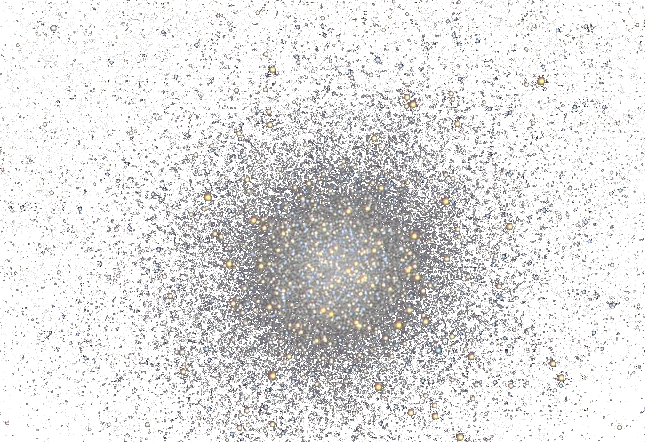
\includegraphics[width=15cm]{ammasso_ercole}};
			\draw[ultra thick] (15,-10.2) rectangle (30,0.2);
			%monsters
			\draw [fill=space,ultra thick] (0,8.5) rectangle (20.5,-1.5);
			\pic at (1,0) {monster01};
			\pic at (8.5,-0.5) {monster02};
			\pic at (13.5,-0.5) {monster03};
			\pic at (6.5,5) {monster04};
			%dida
			\draw [fill=dida,thick] (17.3,7.5) rectangle (29,3.5);
			\node at (22.7,6.5) {\textcolor{black}{\fontsize{23}{24}\selectfont Ah! Il vero ammasso di}};
			\node at (23.2,5.5) {\textcolor{black}{\fontsize{23}{24}\selectfont Ercole è quello nella foto}};
			\node at (19.8,4.5) {\textcolor{black}{\fontsize{23}{24}\selectfont qui sotto!}};
		\end{scope}
		%
		\begin{scope}[shift={(0,-76.5)}]
			\node at (27,0) () {
\includegraphics[width=3.7cm]{licenza}};
			\node at (18,-0.1) {\textcolor{black}{\fontsize{14}{15}\selectfont Testo e illustrazioni: @ulaulaman - Gianluigi Filippelli}};
		\end{scope}
	\end{tikzpicture}
%
\end{document}
